\section{Implementing FICA in Wireless Sensor Networks}
\label{sec:fits}

Significant changes were necessary to adapt the original Strogatz
coupled-oscillators model for use on wireless sensor nodes.  Because
Strogatz's model is well documented in the literature we offer only a brief
description here.  We then continue this section detailing the challenges
created by assumptions in the model untenable on real systems and describing
our solutions.

\begin{figure}[t]
\begin{center}
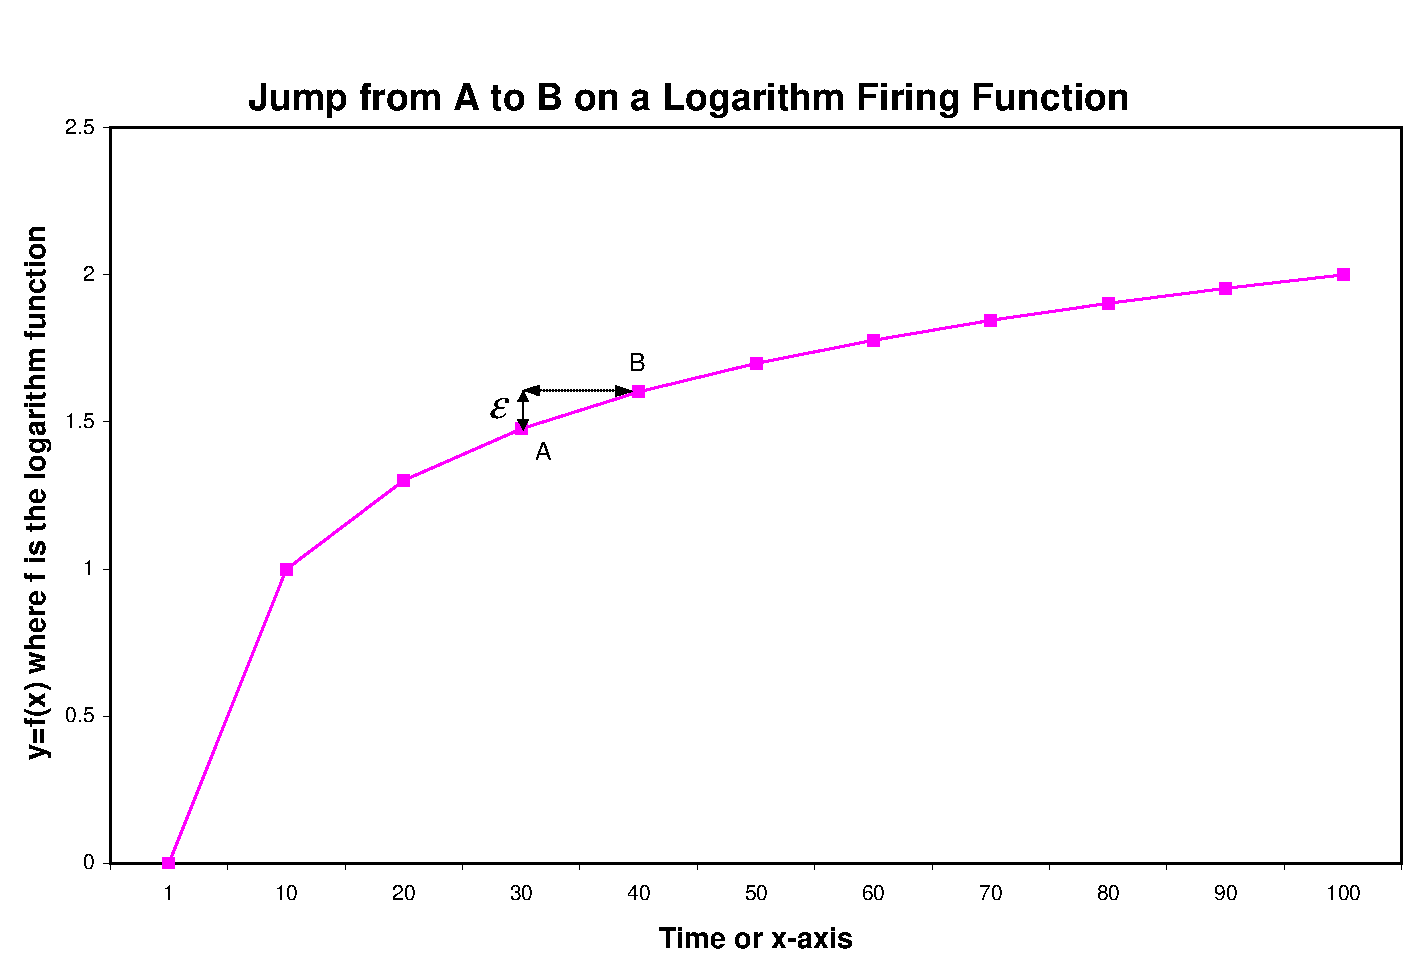
\includegraphics[width=0.9\hsize]{./figures/excelFiringFunc.pdf}
\end{center}
\caption{{\small {\bf A logarithm firing function that displays
a jump from $A$ to $B$ on the curve.}}} 
\label{fig:firingFunc}
\end{figure}

\subsection{The Firefly Synchronization Model}
\label{sec:fireflyModel}

Mirollo and Strogatz extend Peskin's original model for the synchronous
firing of biological oscillators.  Each node in the network is an oscillator
that periodically emits a pulse.  The internal dynamics of the oscillator at
each node, say node $i$, can be generated as a function of a state variable
$x_i(t)$ which takes values within $[0,x_{th}]$, where $x_{th}=1$, is the
threshold value. $x_i(t)$ is a monotonically increasing function that
achieves the threshold value at some time $\tau_i$. Once the threshold is
achieved, the node immediately emits a pulse, $p(t)$ and resets the state
variable to 0, i.e. $x_i(\tau_i^+)=0$.  Mirollo and Strogatz specify that
$x_i$ evolves according to $x_i=f(\phi_i)$, where $f:[0,1]->[0,1]$, is
the \emph{firing function} and it is smooth, monotonic increasing, 
and concave down, i.e., $f'>0$ and $f''<0$.
Here $\phi_i \in [0,1]$ is a phase variable such that, $d\phi / dt = 1/T$,
where T is the cycle period. Furthermore, $\phi_i=0$ when the oscillator is
at its lowest state $x_i=0$, and $\phi_i=1$ at the end of the cycle when
$x_i=1$. Therefore, $f$ satisfies $f(0)=0$, $f(1)=1$.
Fig.~\ref{fig:firingFunc} shows a typical $f$.  The pulses received at each
node will cause an increase to the state variable, thus creating an offset in
the phase of each receiving node.  This effect on the state variable is
called the \emph{coupling} between the transmit and receiver nodes.

Mirollo and Strogatz assume in their model that the oscillators have
identical dynamics, and each is coupled to all the others, and thus has
\emph{all-to-all} communication.  Recent work by Lucarelli and
Wang~\cite{lw04} builds upon this model of pulse coupled oscillators, and
shows that synchronization can be achieved purely on the basis of local
communication, thus discarding the necessity of the all-to-all communication
assumption.


\subsection{The Firing Function}
\label{sec:firingFunc}

The firing function should be monotonically increasing and concave down
according to Mirollo and Strogatz's model.  
Lucarelli and Wang suggest a variety of functions, such as linear, sine, and hyperbolic sine,  
that satisfy this constraint and guarantee synchronization.
Due to the aforementioned resource constraints on the motes, either a very simple linear firing function 
can be selected that does not require floating point arithmetic, or a strategy
is needed to linearize the computation of a non-linear firing function.

The firing function is used to compute the next position, $p_i$ on the 
firing function curve when a pulse or fire is detected. 
Let $(x,y)$\footnote[1]{
We implore the reader to resist the temptation of confusing the $x$ used 
to denote the value on the x-axis in this
context with state variable $x_i$ in section~\ref{sec:fireflyModel}. Although
the notation is confusing, we use $x_i$ to represent the state variable
in order to remain consistent with previous literature that documents Mirollo and Strogatz's model.
}
represent the position of $p_i$ before the fire is detected, 
and let $(x',y')$ represent the new position given that the pulse is detected.
It should be noted that $y$ is not stored explicitly since it can be 
computed using the firing function, $y=f(x)$.
According to Mirollo and Strogatz's model, $y'$ is $y+\epsilon$,
and $x'$ is $f'(y')$ where $\epsilon < 1$ and represents a constant increment in the y axis 
(see Fig.~\ref{fig:firingFunc}), and $f'$ is the inverse of the firing function.
Therefore, in order to implement the model, the inverse of the firing 
function also needs to be computed efficiently.  
We refer to $\frac{1}{\epsilon}$ as the \emph{firing function constant} through
the remaining course of this paper. 

We choose a logarithm function as the firing function.  This is because
apriori it seems that a linear function will be too simple and will not provide
accurate synchronization, and secondly because we can outline a simple
way to linearize the function and compute it efficiently given integer-only
arithmetic that available on the MicaZ sensors. The derivative of $log(x)$ provides a convenient way to linearize
the function in the following way:

\begin{equation}
{dy \over dx}log(x) = {dy \over dx} = {1 \over x}
\end{equation}

\begin{equation}
dy = {dx \over x}
\end{equation}

\begin{equation}
dx = x dy
\end{equation}

The derivative allows us to implement the model in one dimension rather 
than two and does not require computing the inverse of the firing function. 
When a fire is detected, the position of the state variable on the
firing function can be computed by simply multiplying the current $x$ value 
by $dy$, where $dy$ represents $\epsilon$, the firing function constant.
Thus $x' = dx + x$ and $y' = dy + y$.
Evidently, the accuracy of this computation is influenced by the magnitude
of the $dy$ jumps.  In particular, the smaller the $dy$ values, the more accurate will
be the $dx$ value computed. Since the original model defines $\epsilon$ to be
small, specifically $\epsilon < 1$, inaccuracies introduced by using large values
of $dy$ are not a concern in this scheme.


\begin{figure*}[t]
\begin{center}
\begin{tabular}{|p{5cm}|p{3cm}|p{3cm}|p{3cm}|} 
\hline
& {\bf Mirollo and Strogatz} & {\bf Lucarelli and Wang} & {\bf FICA} 
\\ \hline
  {\em \begin{center} Communication Assumptions \end{center}} & 
  {Perfect links and all-to-all communication} & 
  {Perfect links but with only local communication required} &
  {Imperfect, lossy links and only local communication feasible}
\\ \hline
  {\em \begin{center} Event Processing Time \end{center}} &
  {None} &
  {None} &
  {Non-zero, and must be kept to minimum to reduce power and interference
  with other application components}
\\ \hline
  {\em \begin{center} Numeric Precision \end{center}} &
  {Infinite} &
  {Infinite} &
  {Limited by processing exigencies and lack of a floating point unit on the
  ATmega128}
\\ \hline
  {\em \begin{center} Oscillator Dynamics \end{center}} &
  {Perfectly stable oscillators} &
  {Perfectly stable oscillators} &
  {Different crystals on different nodes cause skew, and even on a single
  node environmental factors cause changes over time}
\\ \hline
  {\em \begin{center} Communication Delay \end{center}} &
  {None} &
  {None} &
  {Significant.  Scales with network neighborhood size}
\\ \hline
\end{tabular}
\end{center}
\caption{\small {Differing assumptions used in the different Firefly models.
The breakdown of these assumptions on real hardware nodes required changes to
Strogatz's original model.}}
\label{fig-challenges}
\end{figure*}

\subsection{Implications of Implementing in a Wireless Sensor Network}

Our goal was to implement the Strogatz's Firefly Synchronization model on
networks of MicaZ ''motes''.  The MicaZ is a recent addition to the Mica
family of wireless sensor network devices.  It consists of a 7.3~Mhz
ATmega128L processor, 4KB of SRAM, 128KB of Flash memory for code and data,
and a Chipcon 2420 802.15.4/Zigbee-compliant radio operating at 2.4~Ghz.  The
MicaZ also provides a 51~pin expansion connector allowing integration with
external sensors. The MicaZ runs a small, component-based interface called
TinyOS.  

Table~\ref{fig-challenges} summarizes the main assumptions made in 
the firefly based synchronicity models, and compares this with the conditions
under which we implement FICA.
None of the assumptions made by Mirollo and Strogatz's model can be
upheld in a wireless sensor environment. Noise present in the environment
and packet collisions will introduce error in the routing of simultaneous pulse messages 
between nodes.  Backoff delays introduced by the Medium Access Control (MAC) layer, 
and other radio anomalies extend communication delay and introduce a 
large measure of non-determinism in the time of arrival of pulse messages. 
Furthermore, the all-to-all communication assumption is not feasible 
in multihop networks. Therefore, the demonstration by Wang and Lucarelli~\cite{lw04}
that pulse coupled oscillator based synchronicity can still be achieved 
despite relaxing this assumption forebodes well for the goals of this paper.

Sensor mote hardware also plays a role in violating the assumptions of Mirollo and Strogatz's model. 
Crystal oscillators, are influences by factors such as temperature and humidity, 
and are seldom manufactured identically. Therefore, clock skew is unavoidable in 
the sensor motes since they all tick at different rates. 
This will cause synchronization to degrade as clocks drift apart, and the oscillators
no longer have identical dynamics. Precision will therefore decay as more time elapses between 
synchronization pulses. According to a recent study, typical crystal oscillators
are accurate on the order of one part in $10^4-10^6$~\cite{vig92}, that is two nodes' clocks
will drift apart at $1-100\mu$sec per second.

One of the main changes to Mirollo and Strogatz's model that is introduced
in our implementation is communication delay. In order to address this, we introduce
a delay in processing firing events that are detected by one cycle. This allows
us to efficiently process events in batch mode. Further details of this change
and how we implement it are provided in section~\ref{sec:fitsImplementation}.

Limited computational, energy and memory resources on the motes also constrain
the level of complexity and accuracy of computations that can be performed.
In particular, the absence of floating point arithmetic limits the choice
of a firing function.


\subsection{Implementation Strategy}
\label{sec:fitsImplementation}

\begin{figure}[t]
\begin{center}
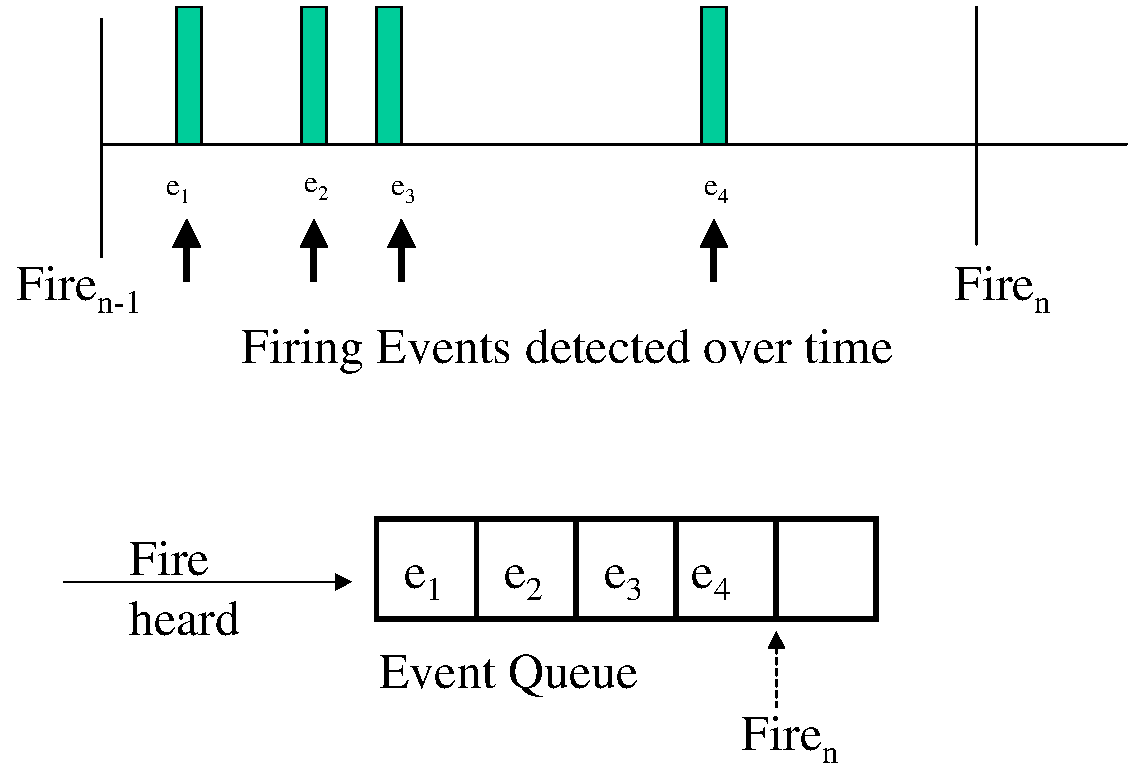
\includegraphics[width=0.9\hsize]{./figures/sortedQueue.pdf}
\end{center}
\caption{{\small {\bf Event Processing: Detected events are stored in a queue sorted by their arrival times and processed at a given time.}}} 
\label{fig:sortedQueue}
\end{figure}

\noindent
In order to address the aforementioned delays introduced by the wireless
sensor network environment, we design an implementation strategy to virtualize time. \\

\noindent
{\bf Processing Events}  \\
In our system each firing event is characterized by 
two messages, the firing message itself and a delay message. 
A firing message contains the sender's local time at
the time it queued the firing message to be sent. A delay message
contains a second timestamp, again using the sender's local
time. The difference between these times represents how long ago the
firing was meant to have occurred. A receiver can then record a firing
event in its own local time by simply subtracting the delay from the
reception time. Each node is assigned a sorted queue to store
detected firing events. The resulting firing event, stored in local time,
is added to the node's sorted queue to be processed later.
All firing events received in one cycle, i.e. received upto a certain amount of 
\emph{idle} time are stored in this queue.  Thus each node remains idle
for a certain period of $\delta(t)$ time, during which it receives and records
firing events. When this idle period is over, the node begins to process the queued events.
Fig.~\ref{fig:sortedQueue} illustrates the queue-based approach of storing
and processing firing events.

Each time a node fires, the next time it will fire can be computed
based on the firing events it detected thus far that are 
stored in the sorted queue.

The tradeoff of the virtualized time strategy is that the response to firing events
is no longer in real time. Firing events detected impact the next firing cycle rather than
the current one. For instance in the first cycle, there are no events in the queue.
Thus, we program the nodes to remain idle by simply storing and processing the events
they detect during this first cycle.

We take a moment to digress to detail a caveat introduced by our hardware
platform. The radio stack on the MicaZ sensor motes, CC2420, does not
permit including the delay message in the same packet as the firing message.
Therefore, two messages are necessary.\\

\noindent
{\bf Computing Next Firing Time}  \\
A node moves closer to firing based on two factors: detecting a firing
and the passing of time. When a firing event is dequeued, the amount of 
elapsed time since the last event recorded is noted.
The represents the time spent waiting without detecting any event. 
This interval is added to the current time, and the magnitude of the jump
on the firing function is computed. This jump is added to the node's 
current time.

In order to implement this, two notions of time need to be tracked:
wall clock time,  which represents the time elapsed between processing
events, as well as the value on the x-axis of the node's current
position on the firing function. \\

\noindent
{\bf 'Ignore-period' For Addressing Pulse Additivity Issues}  \\
Initial experiments showed that on a 15 nodes fully connected graph,
the nodes split into two groups where each individual group achieves synchronicity
amongst its members, but does not achieve synchronicity with the other group.
We believe one reason could be that the additive effect of multiple firings
from the neighboring group is preventing the group from synchronizing with
that group. In order to correct for this \emph{additivity} issue, we 
introduce an \emph{ignore-period} which characterizes the amount of time
during which a node just drops detected events rather than processing
them or storing them in a queue.  Since the ignore-period period may
not be the best solution for the additivity issue, we have implemented
it in a select number of experiments, to determine its effectiveness
in addressing the pulse additivity issues.





